% !TEX encoding = UTF-8
% !TEX program = pdflatex
% !TEX root = relazione.tex
% !TeX spellcheck = it_IT

%----------------------------------------------------------------------------------------
%	PACKAGES AND MISC SETTINGS
%----------------------------------------------------------------------------------------

\documentclass[fleqn,a4paper,11pt]{article}
\usepackage[italian]{babel}
\usepackage[utf8x]{inputenc}
\usepackage[margin=1in]{geometry}
\usepackage[final]{graphicx}
\usepackage[toc,page]{appendix}
\usepackage[nottoc,notlot,notlof]{tocbibind}
\usepackage{amsmath}
\usepackage{amsthm}
\usepackage{wasysym}
\usepackage{stmaryrd}
\usepackage{amsfonts}
\usepackage{booktabs}
\usepackage{xcolor}
\usepackage{colortbl}
\usepackage{xcolor}
\usepackage{xfrac}
\usepackage{url}
\usepackage{listings}
\definecolor{codegreen}{rgb}{0,0.6,0}
\definecolor{codegray}{rgb}{0.5,0.5,0.5}
\definecolor{backcolor}{rgb}{0.98,0.98,0.98}
\definecolor{RoyalBlue}{rgb}{0.25, 0.41, 0.88}
\definecolor{Peach}{rgb}{1.0, 0.9, 0.71}
\definecolor{SeaGreen}{rgb}{0.18, 0.55, 0.34}

\renewcommand{\lstlistingname}{Codice}% Listing -> codice
\renewcommand{\lstlistlistingname}{Frammenti di codice}% List of Listings -> Frammenti di codice

\lstdefinestyle{mystyle}{
    backgroundcolor=\color{backcolor},
    commentstyle=\color{Peach}\ttfamily,
    keywordstyle=\color{RoyalBlue},
    numberstyle=\tiny\color{codegray},
    stringstyle=\color{SeaGreen}\ttfamily,
    basicstyle=\footnotesize\ttfamily,
    breakatwhitespace=false,
    breaklines=true,
    captionpos=b,
    keepspaces=true,
    numbers=left,
    numbersep=5pt,
    showspaces=false,
    showstringspaces=false,
    showtabs=false,
    tabsize=2,
    frame=trbl, % draw a frame at the top, right, left and bottom of the listing
	frameround=ftff, % angolo in basso a destro curvo
	framesep=4pt, % quarter circle size of the round corners,
	inputencoding=utf8x,
    %extendedchars=true,
    %literate={á}{{\'a}}1 {à}{{\`a}}1 {é}{{\'e}}1 {è}{{\`e}}1 {ù}{{\`u}}1 {ò}{{\`o}}1 {ì}{{\`i}}1,
    belowskip=1em,
    aboveskip=1em,
}
\lstset{style=mystyle}

\lstdefinelanguage{JavaScript}
{
  % list of keywords
  morekeywords={ true, false, catch, function, break,	new, class, extends, var, require, switch, return, import, if, while, for, this, View, Text, StyleSheet},
  sensitive=false, % keywords are not case-sensitive
  morecomment=[l]{//}, % l is for line comment
  morecomment=[s]{/*}{*/}, % s is for start and end delimiter
  morestring=[b]' % defines that strings are enclosed in double quotes
}

\lstdefinelanguage{Properties}
{
	% list of keywords
	morekeywords={ true, false, catch, function, break,	new, class, extends, var, require, switch, return, import, if, while, for, this, View, Text, StyleSheet},
	sensitive=false, % keywords are not case-sensitive
	morecomment=[l]{\#}, % l is for line comment
	morecomment=[s]{/*}{*/}, % s is for start and end delimiter
	morestring=[b]' % defines that strings are enclosed in double quotes
}

\lstdefinelanguage{JSON}
{
  % list of keywords
  morekeywords={string, boolean, int, Array, Node, Asset, AssetDetail, Filter, FilterItem},
  sensitive=false, % keywords are not case-sensitive
  morecomment=[l]{//}, % l is for line comment
  morecomment=[s]{/*}{*/}, % s is for start and end delimiter
  morestring=[b] % defines that strings are enclosed in double quotes
}

\lstdefinelanguage{URM}
{
	% list of keywords
	morekeywords={ S, J, T, Z, I},
	sensitive=false, % keywords are not case-sensitive
	morecomment=[l]{//}, % l is for line comment
	morecomment=[s]{/*}{*/}, % s is for start and end delimiter
	morestring=[b]' % defines that strings are enclosed in double quotes
}

\lstdefinelanguage{RDFA}{
	language=html,
	sensitive=true,
	alsoletter={<>=-},
	ndkeywords={
		% General
		=,
		% HTML attributes
		charset=, id=, width=, height=, property=, about=, rel=, rev=, prefix=, vocab=, content=, datatype=
	},
	morecomment=[s]{<!--}{-->},
	tag=[s]
}

\lstdefinestyle{BashStyle}{
  language=bash,
  basicstyle=\small\sffamily,
  numbers=left,
  numberstyle=\tiny,
  numbersep=3pt,
  frame=tb,
  columns=fullflexible,
  backgroundcolor=\color{yellow!20},
  linewidth=0.9\linewidth,
  xleftmargin=0.1\linewidth,
  framexleftmargin=0.2em}

\lstdefinestyle{myJSON}{
    language=JSON,
    basicstyle=\tiny}


% \lstdefinestyle{makefile}{
%   otherkeywords={.SUFFIXES},
%   alsoletter={:},
%   morekeywords=[1]{SUFFIX, CPP_},
%   morekeywords=[2]{vasp:,makeparam:,zgemmtest:,dgemmtest:,ffttest:,kpoints:,clean:},
%   style=global,%
%   morecomment=[l][commentstyle]{\#},%
%   emphstyle={\color{vimvert}},%
%   moredelim=[s][\color{vimvert}]{\$(}{)}%
%   }

\lccode`~=0
\usepackage{caption}
\setlength\abovecaptionskip{.4em}
\setlength\belowcaptionskip{.8em}
\usepackage{hyperref}
\usepackage{titlesec}
\usepackage{tabularx}
%\setlength{\extrarowheight}{5pt}
\usepackage{array}
\newcolumntype{?}{!{\vrule width 0.3mm}}
\usepackage{rotating,booktabs}
\def\MC#1{\multicolumn{1}{c}{#1}}
\usepackage{tikz}
\usetikzlibrary{calc}
\newcommand\HRule{\rule{\textwidth}{1pt}}
\newcommand\LRule{\rule{\textwidth}{.5pt}}
\newcommand\DRule{\rule{\textwidth}{.4pt}\\[\dimexpr-\baselineskip+1mm+2pt] \rule{\textwidth}{2pt}}
\usepackage{titlesec}
\titleformat{\chapter}[hang]
{\normalfont\huge\bfseries}{\chaptertitlename\ \thechapter:}{.3em}{}
%\titlespacing*{<command>}{<left>}{<before-sep>}{<after-sep>}
\titlespacing*{\chapter}
{0pt}{5.5ex plus 1ex minus .2ex}{3.3ex plus .2ex}

\usepackage{fancyhdr}	% Use to set header and footer
\pagestyle{fancy}
% E: Even page, O: Odd page, L: Left field, C: Center field
% R: Right field, H: Header, F: Footer
\fancyhead{} % clear all header fields
\fancyhead[RO,LE]{\textbf{Servivi cognitivi e analisi visiva}}
\fancyfoot{} % clear all footer fields
\fancyfoot[LE,RO]{\thepage}
\fancyfoot[LO,CE]{Marco Romanelli}
\renewcommand{\headrulewidth}{0.4pt}
\renewcommand{\footrulewidth}{0.4pt}

\graphicspath{{../img/}}

\begin{document}

%----------------------------------------------------------------------------------------
%	TITLE PAGE
%----------------------------------------------------------------------------------------
% begin intro
\begin{titlepage}
\begin{center}
	\begin{minipage}{6in}
  		\centering
  		\raisebox{-0.5\height}{
\includegraphics [height=80px]{pollo.png}}
  		\hspace*{1.6in}
  		\raisebox{-0.5\height}{
\includegraphics[height=20px]{logoDM.png}}
  		%\hspace*{.35in}
	\end{minipage}\\[1cm]
% Upper part of the page
\textsc{\LARGE Universit\`a di Padova}\\[.2cm]
\textsc{\large Laurea Magistrale in Informatica}\\[.3cm]
\DRule \\[.5cm]
% Title
{\Large \bfseries Corso di Intelligenza Artificiale} \\[.4cm]
{\huge \bfseries Servivi cognitivi e analisi visiva} \\[.4cm]
{\Large Marco Romanelli} \\[.2cm]
{\footnotesize marco.romanelli.1@studenti.unipd.it} \\
{\footnotesize matricola n. 1106706} \\[1cm]
{\large \today}
\HRule \\[3cm]
\end{center}
\end{titlepage}

%----------------------------------------------------------------------------------------


%----------------------------------------------------------------------------------------
%	DOCUMENT HEADER
%----------------------------------------------------------------------------------------

	%----------------------------------------------------------------------------------------
	%	TOC
	%----------------------------------------------------------------------------------------

	\clearpage
	\tableofcontents
	\newpage

	%----------------------------------------------------------------------------------------
	%	BODY
	%----------------------------------------------------------------------------------------

	% INTRO
	% !TEX encoding = UTF-8
% !TEX program = pdflatex
% !TEX root = relazione.tex
% !TeX spellcheck = it_IT

% INTRODUZIONE
\section{Introduzione}

\subsection{Scopo del progetto}
Il progetto consiste in un'analisi delle principali piattaforme che offrono servizi di \textit{Cognitive Computing},
partendo con una panoramica generale per poi focalizzarsi sull'analisi delle immagini.

\subsection{La teoria computazionale della mente}
Con il termine \textit{Cognitive Computing} si indicano quelle piattaforme di calcolo che comprendo al loro interno servizi
di \textit{machine learning}, ragionamento, analisi del linguaggio naturale, del testo, delle immagini, con lo scopo di simulare
il funzionamento del cervello umano e cercare di migliorare i processi di decisione.
Sviluppare, quindi, un meccanismo unico e universale ispirato alle potenzialità della nostra mente.
Piuttosto che comporre diverse soluzioni separate una dall'altra, si cerca di implementare una teoria computazionale unificata della mente umana.
Allen Newell, un pioniere nell'intelligenza artificiale, in \cite{newell92} la definì come:
\begin{quote}
% a single set of mechanisms for all of cognitive behavior. Our ultimate goal is a unified theory of human cognition
Un insieme unico di meccanismi che include tutti i comportamenti cognitivi. L'obbiettivo finale è una teoria unificata del comportamento umano.
\end{quote}

\subsection{I servizi cognitivi}
% TODO

\subsection*{}
L'articolo procederà come segue: nel Capitolo 2 verranno presentate brevemente le piattaforme prese in esame, illustrando per ognuna i vari sevizi offerti.
Seguiranno poi nei capitoli 3-6 le analisi dettagliate di ciascuna piattaforma, focalizzandosi sull'analisi delle immagini.
Il Capitolo 7 riassume in forma sintetica le funzionalità viste.
Il Capitolo 8 concluderà con le conclusioni dell'autore e alcuni possibili sviluppi di questo lavoro.


	% PANORAMICA
	% PANORAMICA
\section{Panoramica}
Molte fra le maggiori aziende nel settore tecnologico e informatico hanno cominciato a offrire servizi cognitivi.
% Da migliorare
%
Fra queste ne sono state individuate quattro, che offrono un'ampia gamma di sevizi, tariffe diversificate in base all'esigenza e la possibilità di sopportare carichi di lavoro molto ingenti.
I servizi presi in esame saranno, quindi:
\begin{itemize}
\item Microsoft Cognitive Services \cite{microsoft-link} (Microsoft Corporation),
\item Watson Services (Bluemix) \cite{ibm-link} (IBM: International Business Machines Corporation),
\item Amazon Artificial Intelligence \cite{amazon-link} (Amazon.com, Inc)
\item Google Cloud Machine Learning Services \cite{google-link} (Google Inc.)
\end{itemize}

Ognuna di queste suddivide i servizi in macro aeree che possono essere riassunte così: visione artificiale, sintesi vocale, linguaggio naturale, ricerca, tecniche di apprendimento e altro.
Non tutte le piattaforme utilizzando la stessa nomenclatura e i servivi al loro interno possono variare leggermente, ma le aree di interesse coperte sono più o meno queste.
L'area denominata \textit{visione artificiale} include riconoscimento visivo di immagini e video, estrazione di informazioni, riconoscimento volti ed emozioni.
Con \textit{sintesi vocale} vengono indicati quei servizi atti all'elaborazione dell'audio e alla sua trasformazione in testo o in strutture dati adatte all'analisi.
L'area \textit{linguaggio} permette di analizzare ed elaborare il linguaggio naturale, come ad esempio comprendere comandi ed estrapolare informazioni importanti da un dato contesto.
La \textit{ricerca} permette di sfruttare le potenzialità del motore di ricerca offerto dalla compagnia stessa (se presente) o di eseguire ricerche avanzate all'interno di collezioni creati appositamente.
\textit{Tecniche di apprendimento} permette la fruizione di algoritmi e modelli, oltre che alla loro creazione, per l'apprendimento automatico ed approfondito.
La macro area \textit{altro} comprende tutti quei servizi che non ricadono nelle aree precedentemente descritte, come ad esempio sistemi di raccomandazione o altro.
Infine, la tabella \ref{tab-macro-aree} riassume con i servivi offerti (ad alto livello) da ogni piattaforma, inseriti nelle macro aree di riferimento.

E' necessario aggiungere, tuttavia, che questa classificazione vuole fornire solamente una visone generale e grandi linee dei servizi disponibili e non vuole essere esaustiva.
Per l'offerta completa si rimanda alle rispettive documentazioni. Inoltre, l'assenza di voci in una macro area per una certa piattaforma non esclude la presenza di relativi servizi; potrebbero essere, infatti, presenti sotto altri nomi, piattaforme, framework o comunque presenti negli altri servizi.
%
%
\begin{table}[!h]
\centering
{\scriptsize
\begin{tabularx}{.9\textwidth}{X?X|X|X|X}
\toprule
Macro aree & Microsoft Corporation & IBM & Amazon.com, Inc & Google Inc.\\ \hline
\midrule                           
\multicolumn{1}{l?}{Visione artificiale}
& Computer Vision API, Content Moderator, Emotion API, Face API, Video API
%& Computer Vision API & & &\\
%& Content Moderator & & &\\
%& Emotion API & & &\\
%& Face API & & &\\
%& Video API & & &\\
& Visual Recognition
& Amazon Rekognition
& Video Intelligence API, Vision API \\ \hline
\multicolumn{1}{l?}{Sintesi vocale}
& Bing Speech API, Custom Speech Service, Speaker Recognition API
& Speech to Text, Text To Speech
& Amazon Polly
& Speech API \\ \hline
\multicolumn{1}{l?}{Linguaggio naturale}
& Bing Spell Check API, Language Understanding Intelligent Service, Linguistic Analysis API, Text Analytics API, Translator API, Web Language Model API
& AlchemyLanguage, Conversation, Dialog, Document Conversion, Language Translator, Natural Language Classifier, Natural Language Understanding, Personality Insights, Retrieve and Rank, Tone Analyzer
& Amazon Lex
& Natural Language API, Translation API \\ \hline
\multicolumn{1}{l?}{Ricerca}
& Bing Autosuggest API, Bing Image Search API, Bing News Search API, Bing Video Search API, Bing Web Search API, Academic Knowledge API, Knowledge Exploration Service
& Discovery, Discovery News, 
& -
& - \\ \hline
\multicolumn{1}{l?}{Apprendimento}
& -
& -
& Amazon Machine Learning, Apache Spark su Amazon EMR
& Machine Learning Engine \\ \hline
\multicolumn{1}{l?}{Altro}
& Entity Linking Intelligence Service, QnA Maker, Recommendations API
& Tradeoff Analytics
& -
& Jobs API \\ \hline
\end{tabularx}}
\caption{Tabella riassuntiva dei servizi offerti, raggruppati per macro aree}
\label{tab-macro-aree}
\end{table}
%

	% MICROSOFT
	% MICROSOFT
\section{Microsoft Cognitive Services: Computer Vision API}
Per quanto concerne il riconoscimento delle immagini, Microsoft offre le \textit{Computer Vision API} \cite{microsoft-api}, che spaziano dal riconoscimento dei volti all'analisi delle caratteristiche cromatiche dell'immagine.

In base allo scopo per cui si vuole analizzare l'immagine, il servizio mette a disposizione diversi metodi per ottenere le informazioni desiderate:

\paragraph{Tagging} Le API ritornano un insieme di etichette (in formato JSON) che descrivono gli oggetti presenti nell'immagine, come oggetti, esseri viventi, azioni, paesaggi; per ogni etichetta viene anche fornito il livello di \textit{confidence} (affidabilità). I tag non sono in alcun modo organizzati fra loro e non esiste nessun tipo di ereditarietà.
Nel caso un tag sia ambiguo viene fornito in aggiunta un \textit{hint} che ne spiega il contenuto.
Al momento la sola lingua supportata è l'inglese.

\paragraph{Classificazione} L'immagine viene classificata in categorie che seguono una tassonomia con ereditarietà di tipo padre-figlio. Questa tassonomia prevede 86 categorie\footnote{\url{https://www.microsoft.com/cognitive-services/en-us/Computer-Vision-API/documentation/Category-Taxonomy}} e classifica gli elementi visivi in modo più o meno specifico.

\paragraph{Identificazione del tipo} E' possibile classificare l'immagine come in bianco o nero o a colori, se è un disegno o se è del tipo \textit{clip-art}; in quest'ultimo caso viene fornito un livello di qualità dell'immagine, compreso fra 0 e 3.

\paragraph{Riconoscimento volti} Riconosce i volti umani e restituisce la posizione (coordinate) di questi all'interno dell'immagine, come anche età e sesso della persona.

\paragraph{Contenuto personalizzato} Ideato per raffinare la tassonomia a 86 categorie utilizzando informazioni specifiche sul dominio. Attualmente è supportato solamente il riconoscimento dei volti delle persone famose.

\paragraph{Generazione di descrizioni} Genera una lista di frasi (in lingua inglese) che descrivono il contenuto dell'immagine, ordinate secondo un livello di affidabilità calcolato per ogni descrizione.

\paragraph{Estrazione colori} Identifica i colori analizzandoli in tre contesti: di sfondo, in primo piano e d'insieme; i colori sono raggruppati in 12 colori predominanti. Classifica le immagini fra in bianco e nero e a colori.

\paragraph{Riconoscimento contenuti non adatti ai minori} Riconosce materiali pornografici e contenuti osé in generale. Può essere impostato un livello per il filtro.

\paragraph{Riconoscimento del testo (OCR)} Rileva il testo presente nell'immagine e lo trasforma in un flusso di parole, ruota l'immagine se necessario per rendere il testo orizzontale e fornisce le coordinate per ogni parola. Al momento sono supportati 21 linguaggi, fra cui l'inglese, l'italiano, il francese, il tedesco e lo spagnolo.

L'accuratezza del riconoscimento dipende dalla qualità dell'immagine ed eventuali errori possono essere causati da immagini sfuocate, scrittura a mano, testo troppo piccolo, ecc.
   
\paragraph{Creazione anteprime} Un'anteprima è una rappresentazione dell'immagine in scala ridotta. L'immagine viene prima analizzata e poi ritagliata secondo la ``regione di interesse'' (ROI); il rapporto dell'immagine (\textit{aspect ratio}) può essere impostato secondo le proprie preferenze.

\subsection{Tariffe} Due tipologie di piani:
\begin{itemize}
\item Gratuito: fino a 5000 chiamate al mese, massimo 20 chiamate al minuto;
\item Standard: 0,015\$ a chiamata, fino a 10 TPS.
\end{itemize}


	% IBM
	% IBM
\section{IBM Developer Cloud: Visual Recognition}
Il servizio di Visual Recognition\cite{ibm-api} utilizza tecniche e algoritmi di \textit{deep learning} per identificare scene, oggetti, visi di persone nell'immagine che viene fornita come input al servizio. Permette, inoltre, la creazione e l'addestramento di un classificatore personalizzato per l'identificazione di elementi in base alle necessità dello sviluppatore.

\paragraph{Classificazione} Per ogni immagine sottoposta a classificazione viene fornito in riposa una lista di coppie classe-punteggio per ogni classificatore selezionato. Il punteggio è compreso in un intervallo $0-1$, dove un valore maggiore indica una probabilità più alta che la classe descriva l'immagine; la soglia di default perché un valore sia ritornato da un classificatore è $0,5$.
Le classi sono organizzate in categorie e sotto-categorie dove il livello più astratto comprende categorie quali animali, persone, cibo, sport, natura, eccetera.

Le lingue sopportate\footnote{Al momento della stesura di questo documento.} nella risposta sono l'inglese, spagnolo, arabo o giapponese. 

\paragraph{Riconoscimento dei volti} Analizza i volti presenti l'immagine e ne deriva alcune informazioni, come età stimata, sesso o nome del personaggio famoso (nel caso ci sia). Anche in questo caso viene fornito un punteggio (nell'intervallo $0-1$) atto ad indicare una maggiore probabilità di correlazione.

\paragraph{Classificatore personalizzato} Permette di creare un nuovo classificatore e di addestrarlo su un dato insieme di immagini. Queste sono inviate in un file compresso e devono comprendere o due immagini d'esempio positive o una positiva e una negativa. L'insieme contente le immagini d'esempio positive serve a creare le classi che definiscono il nuovo classificatore. Il complementare definisce invece quello che il classificatore \textit{non} deve essere; le immagini d'esempio negative non devono contente i soggetti presenti nelle immagini positive.

Se, ad esempio, si volesse creare un classificatore ``frutta'' si potrebbe utilizzare un file compresso contente immagini di pere, uno contente immagini di mele e uno con immagini di banane.
Per le immagini d'esempio negative si potrebbero utilizzare immagini di verdure.

\paragraph{Collezioni} Questa funzione\footnote{Questa funzione è ancora in fase BETA} permette di creare una nuova collezione, aggiungere immagini a questa e utilizzare la \textit{Similarity Search} per cercare immagini simile all'interno della collezione.

\paragraph{Note per la privacy} Per default, tutte le immagini e le informazioni inviate vengono salvate e utilizzate per migliorare il servizio. Per evitare questo è necessario impostare diversamente il parametro \textsf{X-Watson-Learning-Opt-Out} in ogni richiesta inviata.

\subsection{Tariffe}
Il piano gratuito prevede la possibilità di:
\begin{enumerate}
\item classificare 250 immagini al giorno,
\item addestrare un solo classificatore personalizzato con massimo 5000 immagini.
\end{enumerate}
Il piano \textit{standard} prevede:
\begin{enumerate}
\item per la classificazione: $0,002$ dollari a immagine,
\item per il riconoscimento volti: $0,004$ dollari a immagine,
\item per l'addestramento classificatore: $0,10$ dollari a immagine,
\item per la classificazione con classificatore personalizzato: $0,004$ dollari a immagine.
\end{enumerate}




	% AMAZON
	% AMAZON
\section{Amazon Artificial Intelligence}
Amazon Rekognition \cite{amazon-api} è il servizio di Amazon che permette di riconoscere oggetti, volti, scene, nelle immagini e molto altro.
Inoltre permette l'integrazione con le altre piattaforme offerte da Amazon, come Amazon S3, AWS Lambda e altri servizi AWS.

\subsection{Prerequisiti}
Caratteristiche immagini:
\begin{itemize}
\item Metodo: dati grezzi (stream application/octet) o oggetto Amazon S3.
\item Formati supportati: PNG, JPEG.
\item Caratteristiche minime: 80x80 pixel. 
\item Dimensione massima: 5 MB (dati grezzi), 15 MB (oggetto Amazon S3).
\item Massimo numero di immagini per collezione: un milione.
\end{itemize}
Altro:
\begin{itemize}
\item Disponibilità: Stati Uniti orientali, Stati Uniti occidentali, Europa.
\end{itemize}

\subsection{Amazon Rekognition}
Prima di descrivere cosa si può fare o meno con Amazon Rekognition, è necessaria fare una distinzione; le operazioni fornite dal servizio si suddividono in due categorie:
\begin{itemize}
\item Operazioni volatili (Non-storage API operations): le operazioni in questo gruppo non salvano alcuna informazione sui server Amazon.
\item Operazioni persistenti (Storage-based API operations): l'utilizzo di queste operazioni comporta il salvataggio di alcuni metadati sui server.
Ad esempio nella ricerca di un volto viene salvata la rappresentazione vettoriale dei volti rilevati (mentre l'immagine di partenza no).
\end{itemize}

\paragraph{Rilevamento scene e oggetti} Permette di rilevare automaticamente oggetti, come ad esempio veicoli, alberi, animali e con il relativo punteggio
(\textit{confidence score}) che ne indica il grado di affidabilità (probabilità che sia corretto).
Permette, inoltre, il riconoscimento di scene (una spiaggia o un tramonto), eventi (matrimoni, feste di compleanno) e concetti astratti (serata, paesaggio, natura).
%Questa operazione (\textit{DetectLabels}) non salva alcuna informazione sul server.

\paragraph{Analisi volti} Permette il riconoscimento di volti all'interno dell'immagine, la loro localizzazione spaziale e l'analisi di attributi facciali come
il sesso, l'eta, emozioni, se la persona sta sorridendo, se ha gli occhi aperti, presenza o assenza di barba/baffi, eccetera
\footnote{Per una lista esaustiva si faccia riferimento alla documentazione ufficiale all'indirizzo: \url{http://docs.aws.amazon.com/rekognition/latest/dg/API_Types.html}.}.
La localizzazione avviene tramite un immaginario rettangolo (sotto forma di coordinate $(x, y)$ degli angoli) che circonda ogni viso rilevato e dei punti di rifermento su elementi come il naso,
gli occhi, le orecchie, la bocca, ecc.
Naturalmente, gli algoritmi di riconoscimento sono più affidabili in presenza di visi rivolti frontalmente e potrebbero non riconoscere (o farlo con un punteggio inferiore) visi oscurati
o se rivolti non frontalmente.
%Questa operazione (\textit{DetectFaces}) non salva alcuna informazione sul server.

\paragraph{Confronto volti} A differenza del metodo precedente, questo permette di misurare la probabilità che due volti siano la stessa persona; un punteggio associato ad ogni confronto
aiuta a valutarne il risultato.
Da un'immagine \textit{sorgente} contente un volto, questo viene confrontato con il volti presente nelle immagini \textit{destinazione}.
Anche in questo caso vengono forniture le coordinate spaziali di un immaginario rettangolo che circonda i visi che sono stati rilevati, assieme al grado di sicurezza che quel rettangolo contenga veramente un volto.
%Questa operazione (\textit{CompareFaces}) non salva alcuna informazione sul server.

\paragraph{Riconoscimento volti} Per trovare un volto all'interno di una collezione di immagini. Per prima cosa è necessaria la creazione di una collezione per il salvataggio dei volti, rappresentati come vettore di attributi.
Successivamente si fornisce al servizio un'immagine che provvederà alla ricerca di volti simili all'interno della collezione precedentemente creata.
Per ogni volto restituito viene associato, al solito, un livello di affidabilità la posizione del volto all'interno dell'immagine.


\subsection{Tariffe}
Il piano gratuito prevede ogni mese, per i primi 12 mesi, di:
\begin{itemize}
\item analizzare 5000 immagini,
\item memorizzare 1000 metadati facciali.
\end{itemize}
Altrimenti:
\begin{itemize}
\item per il primo milione di immagini\footnote{Ogni API che accetta una o più messaggi di input conta come un'immagine elaborata.}: $1$ dollaro ogni $1000$ immagini\footnote{Al mese.};
\item successivi 9 milioni di immagini: $0,80$ dollari ogni $1000$ immagini;
\item successivi 90 milioni di immagini: $0,60$ dollari ogni $1000$ immagini;
\item oltre i 100 milioni di immagini: $0,40$ dollari ogni $1000$ immagini.
\end{itemize}
Inoltre utilizzando le API per il riconoscimento dei volti, il servizio memorizza ogni volta la rappresentazione vettoriale dei volti. Questo comporta dei costi pari a $0,01$ dollari per 1000 metadati memorizzati al mese.  

	% GOOGLE
	% GOOGLE
\section{Google Cloud Machine Learning Services: Cloud Vision API}
Le \textit{Google Cloud Vision API} \cite{google-api} permettono di analizzare un'immagine e classificarla in categorie, rilevare oggetti e volti, cercare parole,
moderare contenuti offensivi e molto altro. Le immagini possono essere caricate assieme la richiesta, oppure utilizzare quelle già presenti nel Google Cloud Storage. 

\subsection{Prerequisiti}
Le immagini passate al servizio devono rispettare i seguenti requisiti:
\begin{itemize}
\item Metodo: dati grezzi (stream application/octet) o tramite Google Cloud Storage URIs.
\item Formati supportati: JPEG, PNG8, PNG24, GIF, Animated GIF\footnote{Viene considerato solo il primo frame.},
BMP, WEBP, RAW, ICO.
\item Caratteristiche minime: 640x480 pixel. 
\item Dimensione massima: 4 MB.
\end{itemize}
Altro:
\begin{itemize}
\item Disponibilità: %Stati Uniti orientali, Stati Uniti occidentali, Europa.
\end{itemize}

\subsection{Analisi}
%TODO 

\subsection{Tariffe}
La Cloud Vision API fornisce diversi metodi per analizzare un'immagine.
Ad ogni metodo corrisponde una tariffa che viene applicata ad ogni utilizzo su un'immagine, chiamato \textit{unità};
se, ad esempio, due metodi sono applicati alla stessa immagine allora ai fini tariffari verranno conteggiati separatamente.
Il prezzo è determinato dal numero di unità per mese e il costo per ogni metodo è indicato per 1000 unità/mese in dollari, come indicato in tabella \ref{google-tariffe}.

\begin{table}[!h]
\centering
{\tiny
\begin{tabularx}{\linewidth}{l?c|c|c|c}
\toprule
Metodo & 1-1 000 unità/mese & 1 001-1 000 000 unità/mese & 1 000 001-5 000 000 unità/mese & 5 000 001-20 000 000 unità/mese \\ \hline
\midrule                           
\multicolumn{1}{l?}{\textsf{Label Detection}} & Gratis & 1,50 & 1,50 & 1,00 \\ \hline
\multicolumn{1}{l?}{\textsf{OCR}} & Gratis & 1,50 & 1,50 & 0,60 \\ \hline
\multicolumn{1}{l?}{\textsf{Explicit Content Detection}} & Gratis & 1,50\footnote{\label{explicit}Gratis se utilizzato assieme a \textsf{Label Detection}}
& 1,50\textsuperscript{\ref{explicit}} & 0,60\textsuperscript{\ref{explicit}} \\ \hline
\multicolumn{1}{l?}{\textsf{Facial Detection}} & Gratis & 1,50 & 1,50 & 0,60 \\ \hline
\multicolumn{1}{l?}{\textsf{Landmark Detection}} & Gratis & 1,50 & 1,50 & 0,60 \\ \hline
\multicolumn{1}{l?}{\textsf{Logo Detection}} & Gratis & 1,50 & 1,50 & 0,60 \\ \hline
\multicolumn{1}{l?}{\textsf{Image Properties}} & Gratis & 1,50 & 1,50 & 0,60 \\ \hline
\multicolumn{1}{l?}{\textsf{Web Detection}} & Gratis & 3,50 & 3,50 & n.d.\footnote{\label{explicit} Contattare Google per maggiori informazioni.} \\ \hline
\multicolumn{1}{l?}{\textsf{Web Detection}} & Gratis & 3,50 & 3,50 & n.d.\textsuperscript{\ref{explicit}} \\ \hline
\end{tabularx}}
\caption{Tariffe per la Cloud Vision API}
\label{google-tariffe}
\end{table}


	% ESEMPI
	% !TEX encoding = UTF-8
% !TEX program = pdflatex
% !TEX root = relazione.tex
% !TeX spellcheck = it_IT

% ESEMPI
\section{Esempi}\label{sec:esempi}
Dopo aver fatto una panoramica su cosa viene analizzato di un'immagine, in questa sezione verranno presentati alcuni esempi di utilizzo.
Sono state quindi individuate alcune funzionalità comuni a tutte le piattaforme: riconoscimento oggetti e ambientazione, riconoscimento di volti (singolo e con più volti).
%%
\subsection{Riconoscimento oggetti e ambientazione}\label{subsec:riconscimento-oggetti-ambientazione}
% TODO
%%
\subsection{Riconoscimento di un volto}\label{subsec:riconscimento-singolo-volto}
In questo confronto lo scopo era quello di verificare le caratteristiche del volto (\textit{landmark}) che l'API era in grado di riconsoscere in un ambiente semplice;
per questo motivo è stata scelta un'immagine di un primo piano di una ragazza\footnote{I diritti dell'immagine sono dei rispettivi proprietari.}.
Come si può notare dai risultati in Figura~\ref{fig:riconscimento-singolo-volto}, tutte le API hanno riconosciuto e identificato correttamente il volto e, a parte
il servizio offerto da IBM, diversi elementi di questo.
Il migliore di questi sembrerebbe essere le API di Google che, tuttavia, non fornisce indicazioni sulla persona specifica (età, sesso).
\begin{figure}[!h]
\begin{center}
	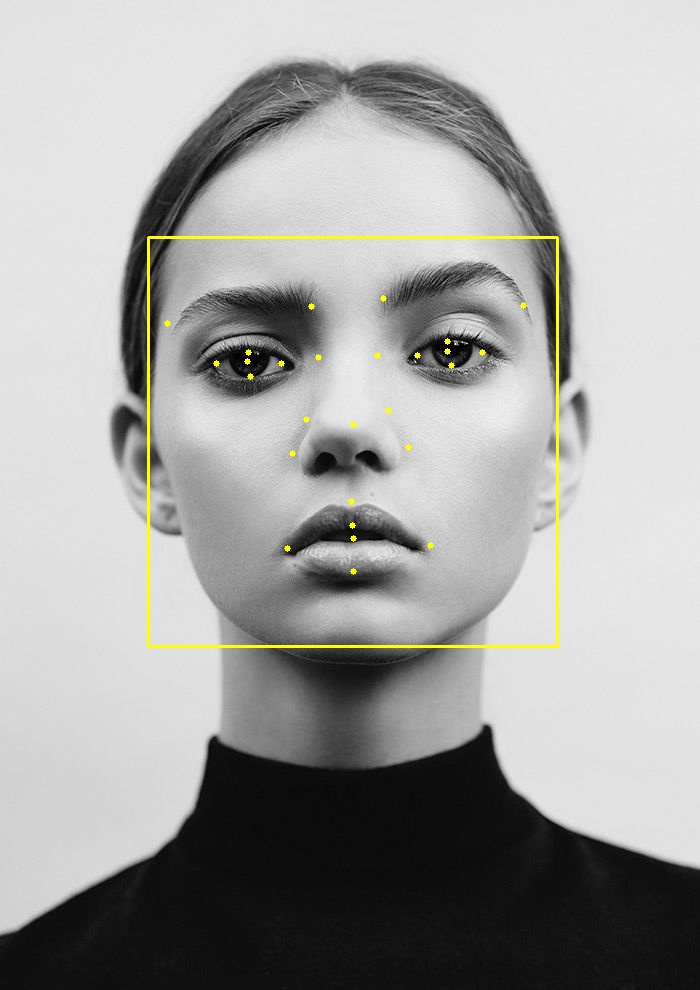
\includegraphics[width=200px,height=282px]{riconoscimento-viso-1/microsoft.jpg}
	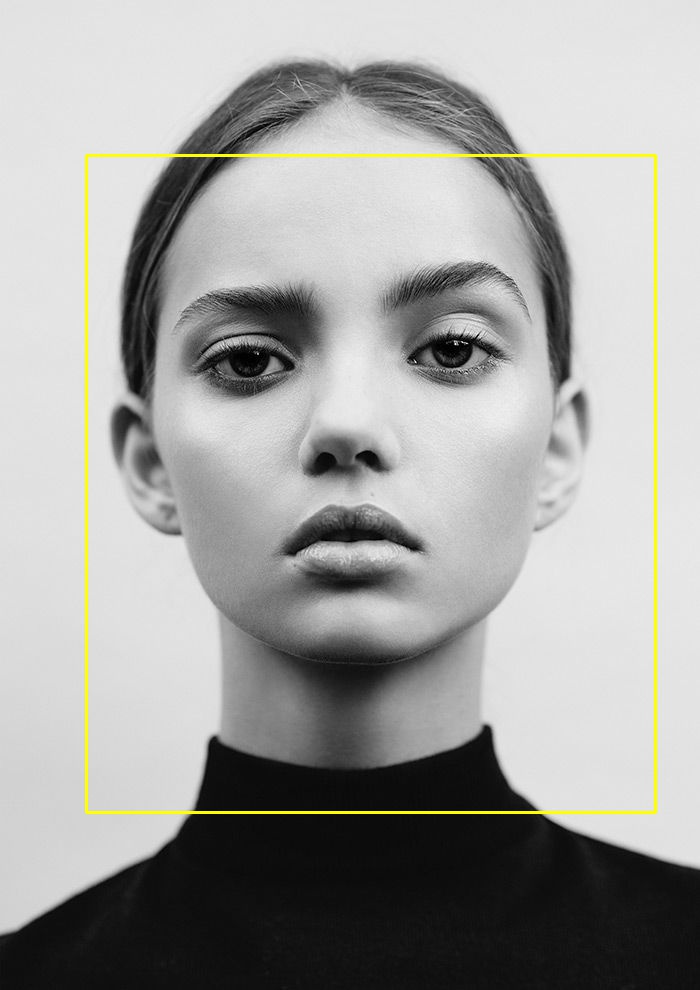
\includegraphics[width=200px,height=282px]{riconoscimento-viso-1/ibm.jpg}
	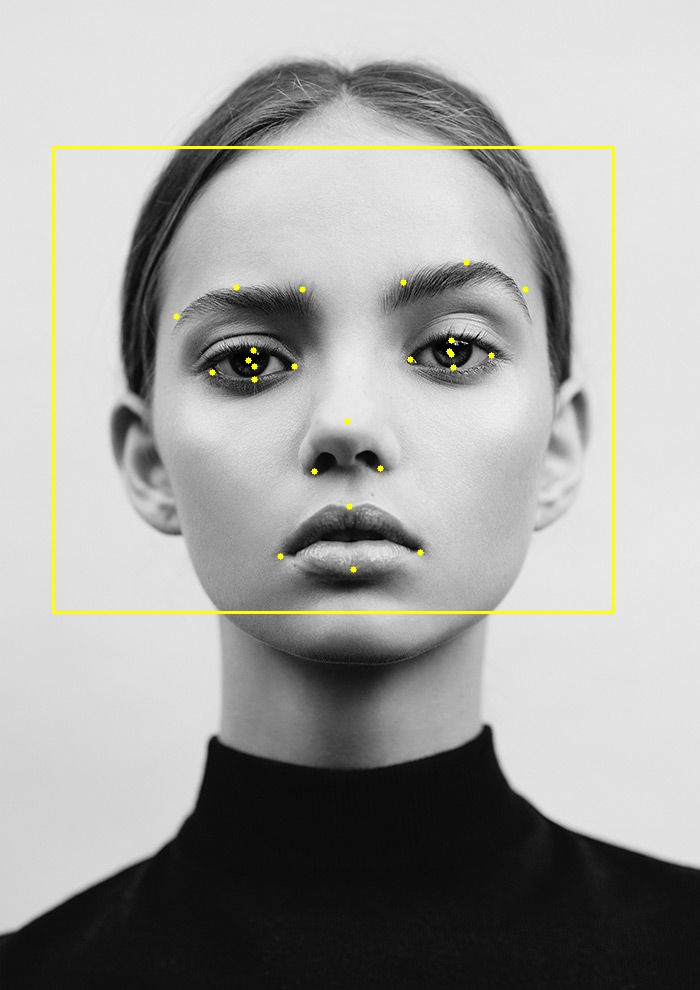
\includegraphics[width=200px,height=282px]{riconoscimento-viso-1/amazon.jpg}
	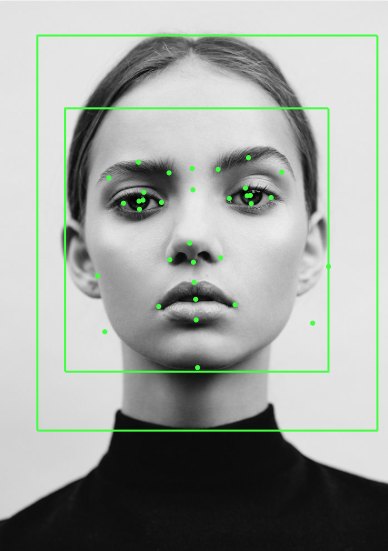
\includegraphics[width=200px,height=282px]{riconoscimento-viso-1/google.png}
{\scriptsize \caption{Riconscimento di un singolo volto utilizzando le API di(da sinistra): Microsoft, IBM, Amazon, Google.}
\label{fig:riconscimento-singolo-volto}}
\end{center}
\end{figure}
%
\subsection{Riconoscimento di più volti}\label{subsec:riconscimento-piu-volti}
%


	% APPLICAZIONI REALI
	% !TEX encoding = UTF-8
% !TEX program = pdflatex
% !TEX root = relazione.tex
% !TeX spellcheck = it_IT

% APPLICAZIONI REALI
\section{Applicazioni reali}\label{sec:applicazioni-reali}
I grafici che seguono rappresentano i modelli tariffari scelti dalle varie piattaforme e mostrano il loro comportamento al variare del ``carico di lavoro''.
Nell'asse delle ascisse si trova, quindi, il numero di immagini (numero di chiamate con un'immagine ogni chiamata) processate al mese,
mentre nell'asse delle ordinate il corrispondente costo in dollari americani\footnote{Regione: West US}.
E' stata scelta questa valuta poiché tutti i servizi coprono il territorio americano (almeno in parte), mentre non è così per altre zone come l'europa;
una valuta come il dollaro, quindi, offre un metro di paragone fra tutti i servizi.

Il primo grafico in ~\ref{fig:grafico1} mostra le differenze di prezzo per riconoscimento di oggetti con un basso carico di immagini, includendo anche i piani gratuiti.
Come si può notare per poche immagini il sevizio offerto da Google non è conveniente, infatti offre gratuitamente solo 1000 chiamate al mese.
Bisogna però ricordare che l'IBM Visual Recognition offre mensilmente il maggior numero di chiamate ma il conteggio è giornaliero.
\begin{figure}[!h]
\begin{center}
	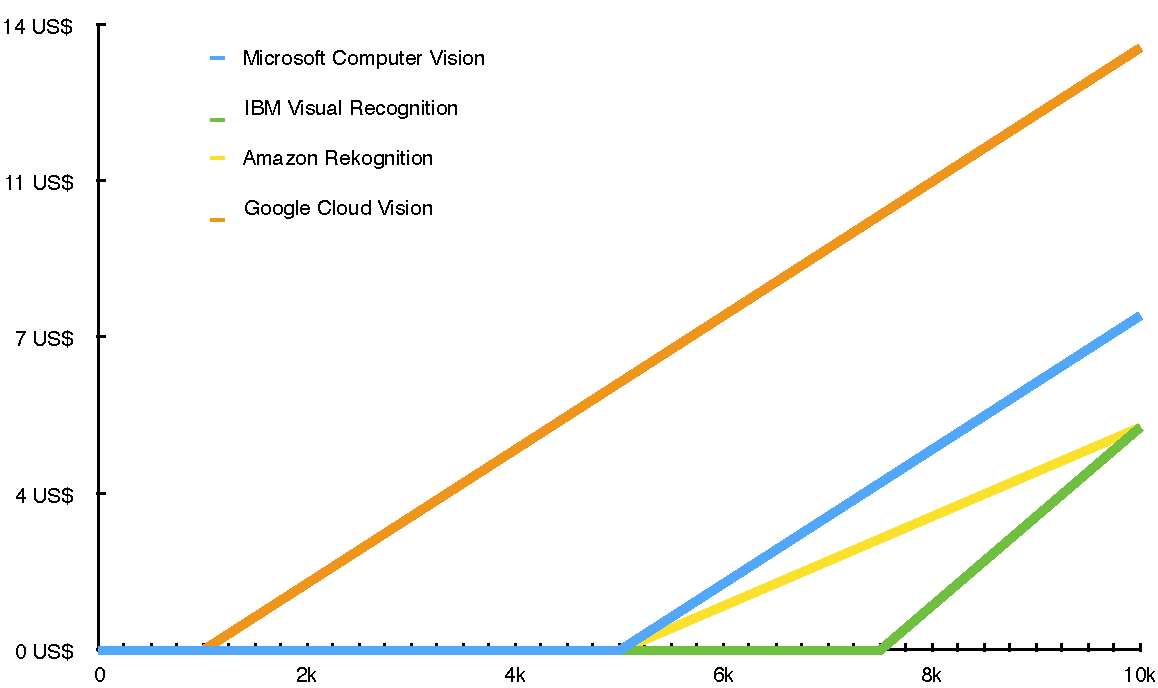
\includegraphics[scale=.4]{grafico1}
{\scriptsize
\caption{Riconoscimento oggetti con piano gratuito (da 0 a 10K di immagini)}
\label{fig:grafico1}}
\end{center}
\end{figure}
%
%
Rimuovendo il piano gratuito iniziale, le tariffe di Google e Microsoft si equivalgono mentre quella più conveniente sembra essere quello di Amazon,
come si evince dal grafico ~\ref{fig:grafico2}.
\begin{figure}[!h]
\begin{center}
	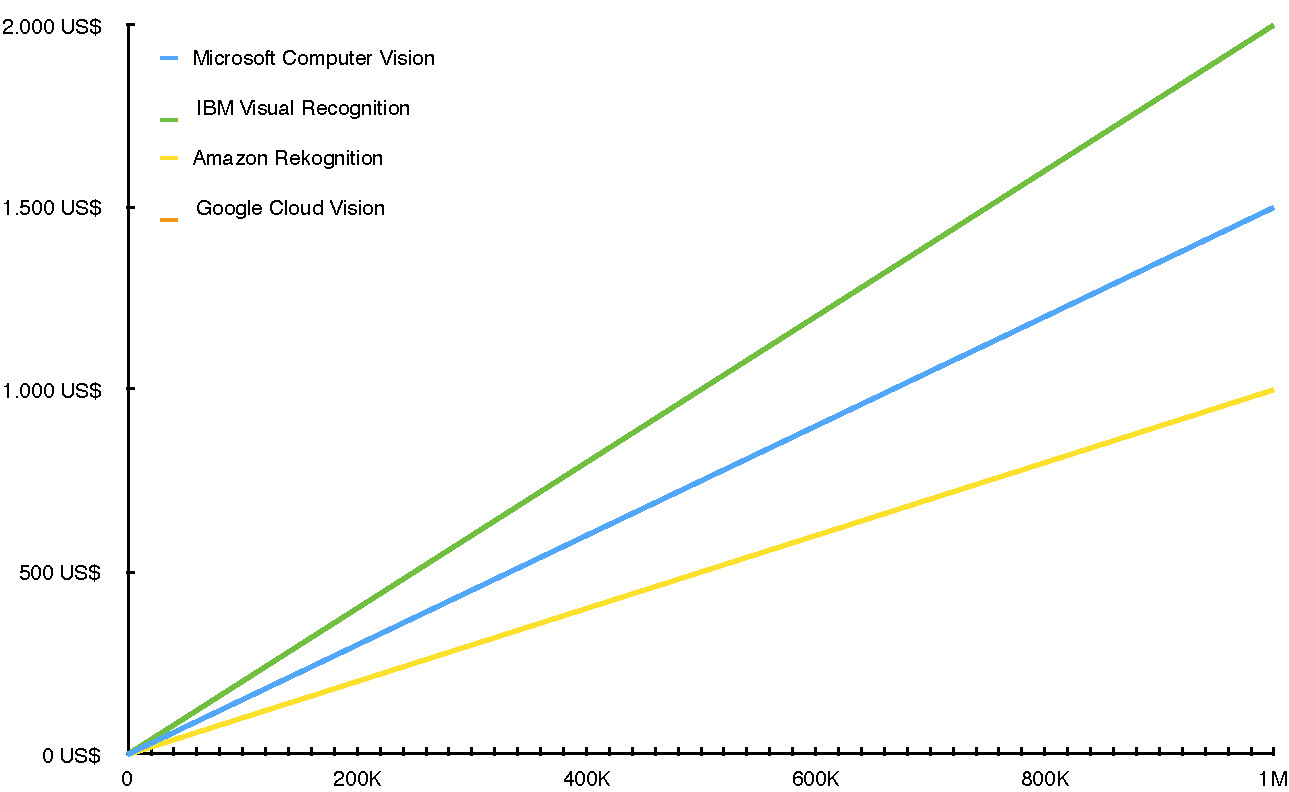
\includegraphics[scale=.4]{grafico2}
{\scriptsize \caption{Riconoscimento oggetti senza piano gratuito (da 0 a 1M di immagini)}
\label{fig:grafico2}}
\end{center}
\end{figure}
%
%
Gli ultimi due grafici, invece, mostrano le tariffe per scenari più reali, con carichi di lavoro dai 50 ai 150 milioni di immagini analizzate al mese.
Il primo ~\ref{fig:grafico3} rappresenta sempre il riconoscimento di oggetti mentre il secondo ~\ref{fig:grafico4} il riconoscimento dei volti.
Questo perché alcuni prevedono costi differenti per il riconoscimento di oggetti e di volti, come ad esempio IBM, dove il costo per la seconda è il doppio,
e Google, quando il numero di immagini al mese superano i cinque milioni.
\begin{figure}[!h]
\begin{center}
	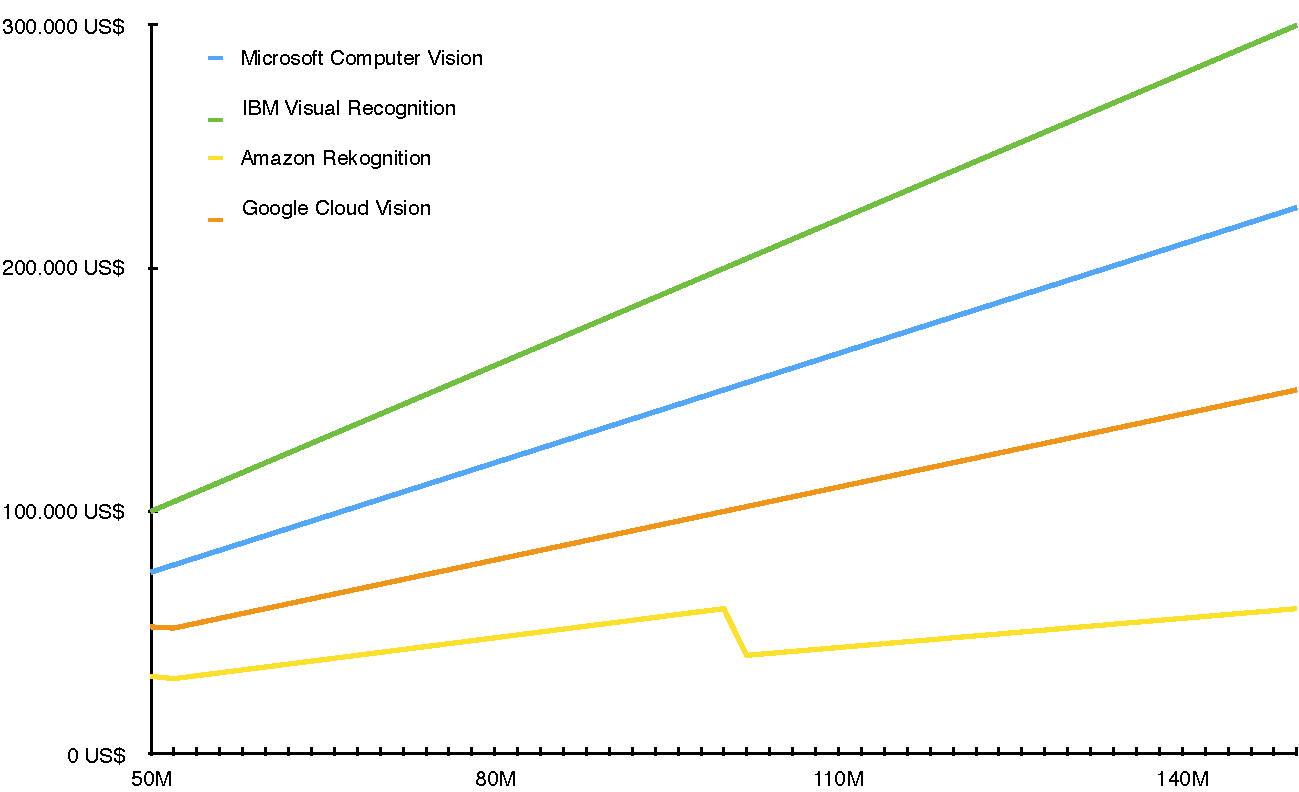
\includegraphics[scale=.4]{grafico3}
{\scriptsize \caption{Riconoscimento oggetti (da 50M a 150M di immagini)}
\label{fig:grafico3}}
\end{center}
\end{figure}
%
\begin{figure}[!h]
\begin{center}
	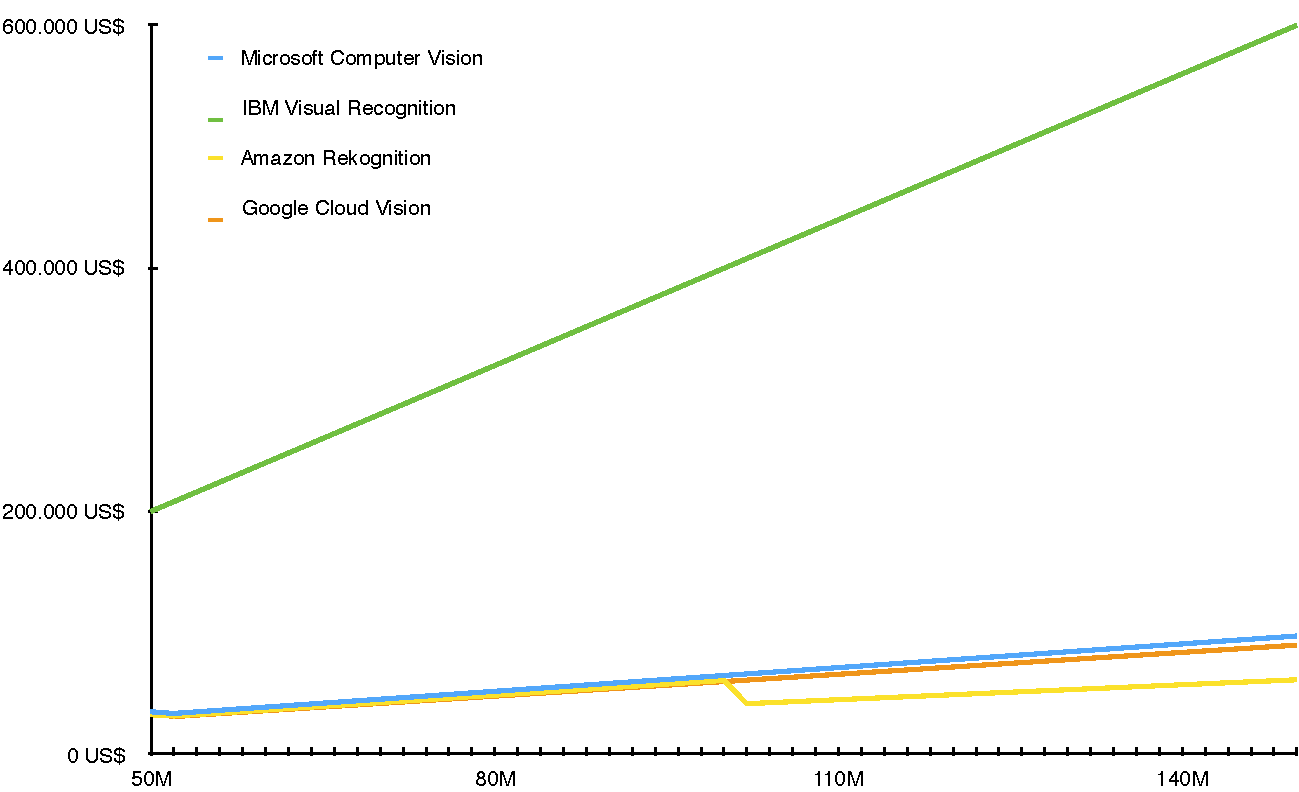
\includegraphics[scale=.4]{grafico4}
{\scriptsize \caption{Riconoscimento volti (da 50M a 150M di immagini)}
\label{fig:grafico4}}
\end{center}
\end{figure}
%
%

Ogni scenario è da considerarsi indipendente dagli altri e rappresenta la stima nel caso peggiore, basandosi su quando scritto nelle relative documentazioni;
per applicazioni concrete, infatti, contattando i fornitori di servizi si potrebbero ottenere tariffe più agevolate.
Inoltre, i costi sono stati calcolati tenendo conto solo delle API analizzate in precedenza, escludendo costi aggiungivi come ad esempio il costo dell'archiviazione.
%
%


	% CONCLUSIONI
	% !TEX encoding = UTF-8
% !TEX program = pdflatex
% !TEX root = relazione.tex
% !TeX spellcheck = it_IT

% CONCLUSIONI
\section{Conclusioni}\label{sec:conclusioni}
In questo lavoro è stato possibile osservare le caratteristiche salienti dell'analisi visiva nell'ambito
dei servizi cognitivi e le possibilità offerte da alcuni fra i maggiori fornitori di queste.
Grazie a questo è possibile, quindi, conoscere i progressi effettuati fino a questo punto,
notare le mancanze che andranno colmate e verso dove si stanno muovendo i prossimi passi.

È opinione dell'autore che i servizi disponibili a tutt'oggi (perlomeno quelli analizzati)
diano buoni, e in alcuni casi anche ottimi, risultati e che permettano di conseguenza
la realizzazione di applicazioni in grado di ineragire con l'ambiente reale con un buon grado di affidabilità
(per sistemi non critici).
%
\subsection{Sviluppi futuri}
Inizialmente si potrebbe includere anche l'analisi di video (che non è stata coperta in questo lavoro).
Il passo successivo sarebbe sicuramente lo studio delle altre macro-aree, come per esempio quella del linguaggio o della ricerca.
Nonostante siano stati inclusi alcuni esempi di utilizzo della API, questi sono molto generici
e danno solo un'idea di massima dei servizi.
Si potrebbe, quindi, includere lo studio di un'applicazione reale (o il più possibile reale), in modo da osservare
il comportamente delle API con un bisogno e problema effettivo.


	\clearpage
	\appendix
	% TABELLE
	% TABELLE
\section{Tabelle riassuntive}
Per riassumere, vengono presentate ora alcune tabelle con i punti salienti per ogni piattaforma.
La tabella \ref{tab-riass-funzionalita} illustra le funzionalità di ogni servizio, in relazione alle API per l'analisi visiva di immagini.
In tabella \ref{tab-riass-tariffe} vengono illustrate le tariffe per ogni servizio (si veda la sezione relativa ad ogni piattaforma per le informazioni dettagliate).

\begin{table}[!h]
\centering
{\tiny
\begin{tabularx}{\linewidth}{l?c|c|c|c}
\toprule
Funzionalità & Microsoft Computer Vision & IBM Visual Recognition & Amazon Rekognition & Google Vision \\ \hline
\midrule                           
\multicolumn{1}{l?}{Riconoscimento oggetti} & \checkmark & \checkmark & \checkmark & \checkmark \\ \hline
\multicolumn{1}{l?}{Riconoscimento scene} & \checkmark & \checkmark & \checkmark & \checkmark \\ \hline
\multicolumn{1}{l?}{Creazione di un classificatore} & & \checkmark & &  \\ \hline
\multicolumn{1}{l?}{Riconoscimento colori} & \checkmark &  &  & \checkmark \\ \hline
\multicolumn{1}{l?}{Riconoscim. tipo imm.} & \checkmark &  &  & \\ \hline
\multicolumn{1}{l?}{Riconoscimento volti} & \checkmark & \checkmark & \checkmark & \checkmark \\ \hline
\multicolumn{1}{l?}{Riconoscimento celebrità} & \checkmark & \checkmark &  & \\ \hline
\multicolumn{1}{l?}{Generazione descrizioni} & \checkmark &  &  & \\ \hline
\multicolumn{1}{l?}{Ric. nudità/violenza} & \checkmark&  &  & \checkmark \\ \hline
\multicolumn{1}{l?}{Riconoscimento del testo (OCR)} & \checkmark &  &  & \checkmark \\ \hline
\multicolumn{1}{l?}{Creazione anteprime} & \checkmark &  &  & \\ \hline
\multicolumn{1}{l?}{Riconoscimento loghi/punti interesse} &  &  &  & \checkmark \\ \hline
\multicolumn{1}{l?}{Ricerca di immagini} & solo volti & \checkmark &  solo volti & \\ \hline
\multicolumn{1}{l?}{Confronto fra immagini} & solo volti & \checkmark & solo volti & \\ \hline
\end{tabularx}}
\caption{Analisi delle funzionalità}
\label{tab-riass-funzionalita}
\end{table}
%%
%%
%\begin{table}[!h]
%\centering
%{\tiny
%\begin{tabularx}{\textwidth}{l?c|c|c|c}
%\toprule
%Tipologia di piano & MC Vision & IBM Visual Recognition & Amazon Rekognition & Google Vision\\ \hline
%\midrule                           
%\multicolumn{1}{l?}{Gratuito [chiamate/mese]}
%& 5000
%& \begin{tabular}{@{}c@{}}
%7500 immagini/mese\footnote{Con limite giornaliero di 250.}\\
%1 classificatore con 5000 imm.
%\end{tabular}
%& \begin{tabular}{@{}c@{}}
%5000 \\
%1000 metadati facciali
%\end{tabular}
%& 1000
%\\ \hline
%\multicolumn{1}{l?}{Standard [dollari/chiamata]}
%& $0,0015$
%& \begin{tabular}{@{}c@{}}
%$0,002$ - $0,004$ (classificazione)\\
%$0,10$ a immagine (addestramento)
%\end{tabular}
%& da $0,001$ a $0,0004$
%& da $0,0035$ a $0,0006$
%\\ \hline
%\end{tabularx}}
%\caption{Analisi delle tariffe}
%\label{tab-riass-tariffe}
%\end{table}
%%
%%
\begin{table}[!h]
\centering
{\tiny
\begin{tabularx}{\linewidth}{l?c|c|c|c}
\toprule
Funzionalità & Microsoft Computer Vision & IBM Visual Recognition & Amazon Rekognition & Google Vision \\ \hline
\midrule                  
\multicolumn{1}{l?}{Metodi di input} & raw, URL & raw, URL & raw, AS3O & raw, GCL URIs \\ \hline         
\multicolumn{1}{l?}{Formati supportati} & JPEG, PNG, GIF, BMP & PNG, JPEG & PNG, JPEG
%& JPEG, PNG8, PNG24, GIF, Animated GIF, BMP, WEBP, RAW, ICO \\ \hline
& \begin{tabular}{@{}c@{}}
JPEG, PNG8, PNG24 \\
GIF, Animated GIF\\
BMP, WEBP, RAW, ICO
\end{tabular}\\ \hline
\multicolumn{1}{l?}{Dimensione minima [pixel]} & 50x50 & 224x224 & 80x80 & 640x480\\ \hline
\multicolumn{1}{l?}{Dimensione massima [MB]} & 4 & 2 & 5 o 15 & 4 \\ \hline
\end{tabularx}}
\caption{Requisiti delle immagini fornite alle API}
\label{tab-riass-immagini}
\end{table}

%
%

	% RISULTATI JSON
	% !TEX encoding = UTF-8
% !TEX program = pdflatex
% !TEX root = relazione.tex
% !TeX spellcheck = it_IT

% RISULTATI JSON
\section{Risultati degli esempi}
%
\begin{lstlisting}[style=myJSON,
	caption=Risultato dell'interrogazione a IBM Visual Recognition per volti (figura~\ref{fig:riconscimento-volti}),
	label=lst:risultati-ibm-volti]
[{
  "age": {
   "max": 44,
   "min": 35,
   "score": 0.403753
  },
  "face_location": {
   "height": 111,
   "left": 84,
   "top": 38,
   "width": 75
  },
  "gender": {
   "gender": "MALE",
   "score": 0.5
  }
 },
 {
  "age": {
   "max": 54,
   "min": 45,
   "score": 0.349335
  },
  "face_location": {
   "height": 107,
   "left": 279,
   "top": 72,
   "width": 99
  },
  "gender": {
   "gender": "MALE",
   "score": 0.622459
  }
 }]
\end{lstlisting}


	% BIBLIOGRAFIA
	\clearpage % da cambiare se prima ci sono troppi spazi vuoti
	\bibliography{biblio.bib}
	\bibliographystyle{ieeetr}

	%----------------------------------------------------------------------------------------
	%	END
	%----------------------------------------------------------------------------------------

\end{document}
